In this project, the goal is to label all faces in the given image as mask/no mask. For example,

\begin{figure}[H]
    \centering
    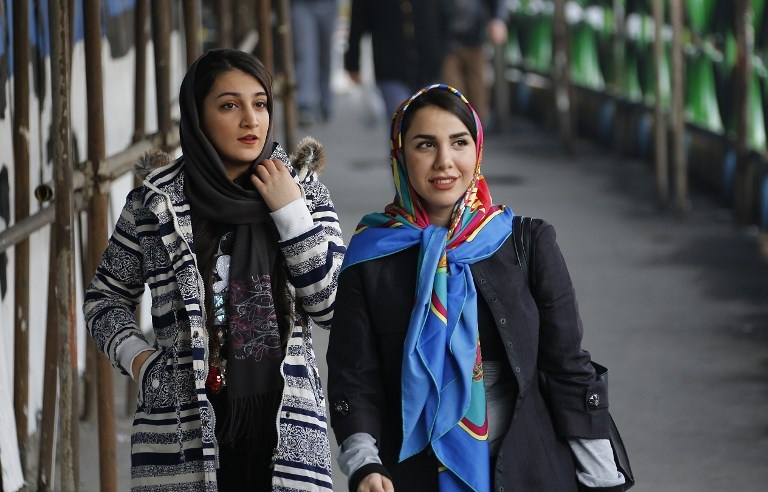
\includegraphics[width=0.7\textwidth]{Orig.jpeg}
    \caption{Original Image}
    \label{fig:Orig}
\end{figure}

\begin{figure}[H]
    \centering
    
\includegraphics[width=0.3\textwidth]{Person1.jpg}
    \caption{First Image}
    \label{fig:First}
\end{figure}

\begin{figure}[H]
    \centering
    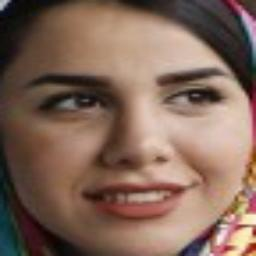
\includegraphics[width=0.3\textwidth]{Person2.jpg}
    \caption{Second Image}
    \label{fig:Second}
\end{figure}

We'll need to determine which of these women is wearing a medical mask.

\subsection{Approach:}
We are interested in labels
\begin{itemize}
    \item face with mask
    \item face no mask
\end{itemize}

We want to train a binary classifier to predict mask true\/false for a given facial image.


The problem with this approach is that face detector might be less accurate on faces with masks on.


We will train a classifier with three classes face\_with\_mask, face\_no\_mask and non-face, and apply it “efficiently” to a larger input image.


\subsection{Train:}
\begin{itemize}
    \item Pre-trained Face Detector:

        Input: frame

	    Output: bounding box around human face
    \item Transfer Learning – fine tune on masked \& non-masked faces (equally distributed)
\end{itemize}


\subsection{Test:}
\begin{enumerate}
    \item Frame from camera/video
    \item Run through Face detector model (inc. masked/non-masked)
    \item Use model to classify Masked  vs. Non-masked
\end{enumerate}


